\newpage
\section{Tenacity Paracity}
In this activity we are going to investigate city geometry parabolas.

\begin{prob} 
Remind me again, what is the definition of a \textit{parabola}?
\end{prob}
\vspace{0.5in}

\begin{prob}
Use the definition of a parabola and taxicab distance to sketch the city geometry parabola when the focus is the point $(2,1)$
and the directrix is $y=-3$. 
\[
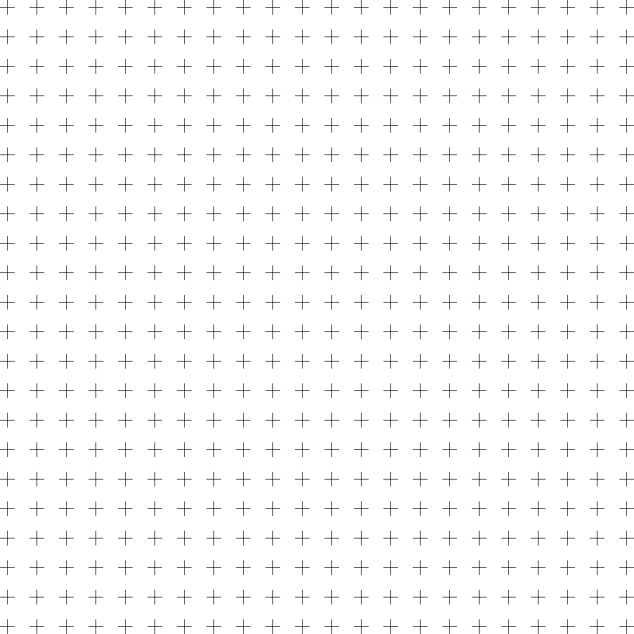
\includegraphics{../graphics/complexPlane}
\]
\end{prob}

\break
\begin{prob}
Comparing geometries with algebra. 
\begin{enumerate}
\item Use coordinate constructions to write an equation for the Euclidean geometry parabola with its focus at $(2,1)$ and its directrix being the line $y=-3$.  (Hint:  No need to simplify.  Just use the definition and set the distances equal to one another.)  
\vspace{0.5in}
\item Use your taxicab distance formula to write an equation for the city geometry parabola with its focus at $(2,1)$ and its directrix being the line $y=-3$.  
\vspace{0.5in}
\item Compare and contrast the two equations.  
\vspace{0.5in}
\item Use algebra of absolute value to show that the graph in the previous problem is the correct graph. 
 (Hint:  Consider three cases: $y>1$, $-3\leq y \leq 1$, and $y<-3$.)
\vfill
\end{enumerate}
\end{prob}

\break

\begin{prob}
Sketch the city geometry parabola when the focus is the point $(4,4)$
and the directrix is $y=-x$.
\[
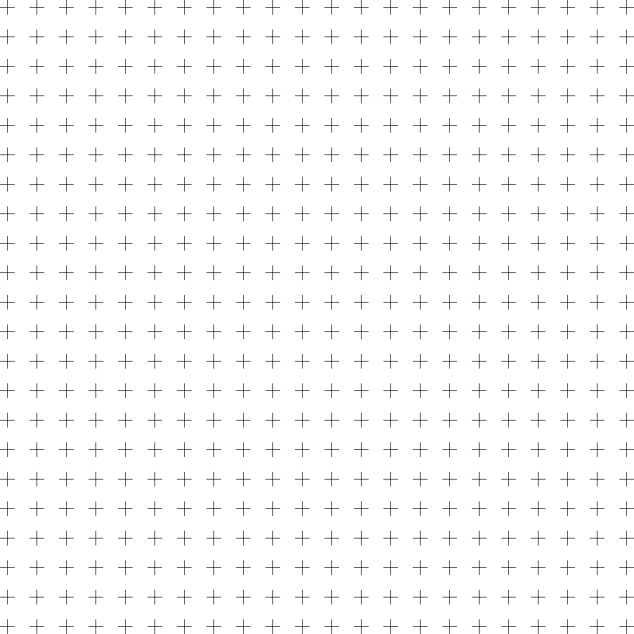
\includegraphics{../graphics/complexPlane}
\]
\end{prob}

\break

\begin{prob}
Sketch the city geometry parabola when the focus is the point $(0,4)$
and the directrix is $y=x/3$.
\[
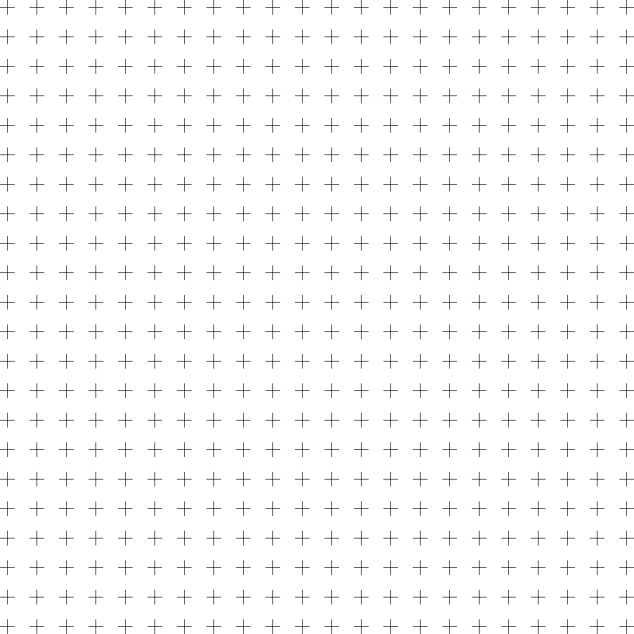
\includegraphics{../graphics/complexPlane}
\]
\end{prob}

\break

\fixnote{Use better numbers here.}
\begin{prob}
Sketch the city geometry parabola when the focus is the point $(4,1)$
and the directrix is $y=3x/2$.
\[
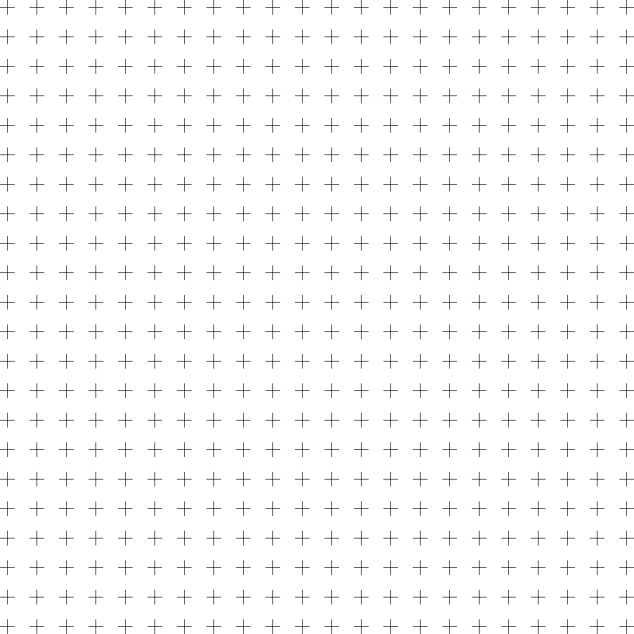
\includegraphics{../graphics/complexPlane}
\]
\end{prob}

\begin{prob}
Explain how to find the distance between a point and a line in city
geometry.
\end{prob}


\begin{prob}
Give instructions for sketching city geometry parabolas.
\end{prob}


